\documentclass[conference]{ieeeconf}

\IEEEoverridecommandlockouts                              % This command is only needed if 
                                                          % you want to use the \thanks command

% Usual setup packages
\usepackage{listings} % For including source code with highlighting
\usepackage{hyperref} % For better hype r-link integration
\usepackage[bottom]{footmisc} % places footnotes at page bottom

% Packages for verbatim text blocks
\usepackage{alltt} % Package for including math in verbatim text
\usepackage{fancyvrb}

% Packages for math symbols and other mathey things
%\usepackage{amsthm}
\newtheorem{theorem}{Theorem}
\newtheorem{lemma}{Lemma}
\newtheorem{claim}{Claim}
\newtheorem{corollary}{Corollary}
\newtheorem{proposition}{Proposition}
\usepackage{amsmath}
\usepackage{amsfonts}
\usepackage{amssymb}
\usepackage{enumerate}

% Packages for including pseudo-code
\usepackage{algorithmicx}
\usepackage{algorithm}
\usepackage{algpseudocode}

% Packages that handle tables, figures and other floats
\usepackage{enumerate}
\usepackage{tabularx}
\usepackage{multirow}
\usepackage{float} % To make floats movable
\usepackage{subcaption}
\usepackage[table]{xcolor}

\usepackage{cite}


% Packages for drawing graphs, FSMs, etc.
\usepackage{pgf}
\usepackage{tikz}
\usetikzlibrary{shapes,arrows,calc,fit,positioning,shapes.symbols,shapes.callouts,patterns,automata,matrix}

% Remove red boxes around refs
\hypersetup{
    colorlinks,
    citecolor=black,
    filecolor=black,
    linkcolor=black,
    urlcolor=blue
}

% ------------------------------ CUSTOM MACROS ------------------------------------
% Nice little macro for adding a comment box. Include incrementing comment numbers.
\newcounter{comcount}
\setcounter{comcount}{0}
\newcommand{\mycomment}[1]
{
\refstepcounter{comcount}
\smallskip\noindent\fbox{\parbox{\linewidth}{\emph{Comment \arabic{comcount}} : \small{#1}}} 
}

\DeclareMathOperator*{\argmin}{\arg\!\min\>}
\newcommand{\amin}[1]{\underset{#1}\argmin}
\DeclareMathOperator*{\argmax}{\arg\!\max\>}
\newcommand{\amax}[1]{\underset{#1}\argmax}

\def\a{\mathbf{a}}
\def\Z{\mathbb{Z}}
\def\R{\mathbb{R}}
\def\N{\mathcal{N}}
\def\estt{\hat{\tau}}
\def\estg{\gamma}
\newcommand{\sig}{\mathcal{S}}
\newcommand{\ceil}[1]{\lceil#1\rceil}
\newcommand{\xm}{x_{\hat{m}}}
\newcommand{\td}{\mathbf{t}}

\begin{document}
\title{Existence of an Equilibrium Strategy for Communication-Free Multi-Robot Task-Assignment}

\author{Anshul Kanakia, Behrouz Touri, and Nikolaus Correll%
\thanks{All authors are with the College of Engineering and Applied Sciences, University of Colorado, Boulder, USA.}%
\thanks{Anshul Kanakia and Nikolaus Correll are with the Dept. of Computer Science. Behrouz Touri is with the Dept. of Electrical Engineering.}%
\thanks{Email format follows: \texttt{firstname.lastname@colorado.edu}}%
\thanks{This research has been supported by NSF grant \#1150223.}%
}

%\author{\authorblockN{Anshul Kanakia and Nikolaus Correll}
%\authorblockA{College of Engineering and Applied Sciences\\
%Computer Science\\
%University of Colorado, Boulder\\
%Boulder -- Colorado, USA\\
%Email: \texttt{first}.\texttt{last}@colorado.edu}
%\and
%\authorblockN{Behrouz Touri}
%\authorblockA{College of Engineering and Applied Sciences\\
%Electrical Engineering\\
%University of Colorado, Boulder\\
%Boulder -- Colorado, USA\\
%Email: behrouz.touri@colorado.edu}}
\maketitle

\thispagestyle{empty}
\pagestyle{empty}

%%%%%%%%%%%%%%%%%%%%%%%%%%%%%%%%%%%%%%%%%%%%%%%%%%%%%%%%%%%%%%%%%%%%%%%%%%%%%%%%
\begin{abstract}
We show that an agent-level threshold strategy for the task-assignment problem in swarm robotics results in system-level equilibrium for collaborative tasks in which individual swarm members do not communicate. While threshold policies have long been used in swarm robotics to model task-assignment, the justification for their use has always been phenomenological in nature; drawing inspiration from threshold based task-assignment models in biological systems such as ant colonies and other social insects. Consequently, we provide the first mathematical explanation for the prevalence of threshold based strategies in both, natural and artificial systems. We formulate task-allocation in swarm robotics as a global game, and then present a proof that shows individual agent threshold-response strategies for task-assignment do indeed result in system-wide equilibrium, under certain conditions. We then show analytically how Gaussian noise in perceiving the stimulus signal leads to sigmoid threshold responses, as are commonly observed in nature. 
\end{abstract}

%%%%%%%%%%%%%%%%%%%%%%%%%%%%%%%%%%%%%%%%%%%%%%%%%%%%%%%%%%%%%%%%%%%%%%%%%%%%%%%%
\section{Introduction}\label{sec:intro}
Task-allocation is central to collaborative tasks such as object transport \cite{Sugawara2012}, oil-spill containment \cite{Beni2005}, firefighting \cite{Kanakia2014}, inspection \cite{Correll2007}, pattern recognition \cite{Beni1993}, and cooperative surveillance. Strategies for task-allocation \cite{Gerkey2004} in a multi-agent system (MAS) vary from deterministic leader-follower coalition algorithms \cite{Chen2011} and more complex market-based approaches \cite{Amstutz2008} to simpler probabilistic algorithms for individually simplistic agents \cite{Dantu2012}. These probabilistic strategies are inspired from biological models of insect colonies. They do not require communication among agents and provide a phenomenological approach to solving the task-assignment problem. Thus far, response-threshold models have provided good agreement with observed behavior in insect colonies and have proved invaluable in engineering solutions to multi-robot collaboration problems. Yet, there has been no theoretical backing for why threshold-based approaches are the better strategies in teams that cannot exchange information.

\begin{figure}[!htb]
\centering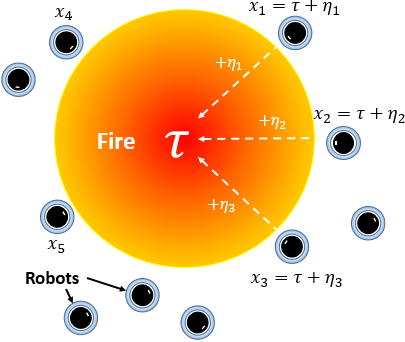
\includegraphics[width=0.9\columnwidth]{../figures/globalgamesetup.png}
\centering\caption{A multi-robot firefighting scenario set up as a global game. Each player's imperfect estimate of the task is represented by $x_i$, a sum of the global magnitude parameter-$\tau$ and noisy sensor measurements-$\eta_i$.}\vspace{-10px}\label{fig:ggsetup}
\end{figure}

We show in this paper that a response-threshold strategy for a broad class of task-assignment problems, under communication constraints  and noisy sensing, results in unique system-wide equilibrium conditions such that no individual agent will receive a better utility by deviating from their strategy to act based on some threshold value $\td$. To prove this statement we employ a sub-class of Game Theory called \emph{global games}, first introduced by Carlsson and Van Damme in 1993 \cite{Carlsson1993}. Global games have been substantially generalized over the years to study and model different phenomena in economics such as pricing debt, currency crisis, and bank runs, and we strongly believe they can be further applied to the analysis of task-assignment in MASs. See \cite{Morris2000} and the references therein for more details on applications of global games.

Collaborative tasks for MASs can be formally defined as global games with the property of \emph{concurrent benefit}. Informally, concurrent benefit is an attribute of a collaborative task where a certain minimum number of agents is needed to solve a task; if this number is not reached, agents which try nevertheless waste their efforts. In addition, the exact number of agents required to successfully complete the task is unknown and varies over time due to numerous, complex physical parameters. Many collaborative tasks---particularly those seen in biological systems---exhibit the property of concurrent benefit ranging from surveillance and coordinated defense of enclosed areas like termite mounds and honey bee hives \cite{Breed1990} to collective transport of heavy objects and even containment of oil spills and forest fires. The probability of success depends, non-linearly, on the average number of agents assigned to that task. For example, 5--10 ants may be insufficient to lift a heavy object such as a small rock or twig and will waste a considerable amount of energy and time in trying, but 12 or more ants might accomplish the task successfully. Similarly, in a MAS setting, consider the task of collaborative firefighting. To contain a large fire, it is insufficient (and inefficient) for a single agent to start putting out the fire without waiting for backup. But the rate of fire containment increases quickly by adding just a few more agents to the group, which illustrates the property of concurrent benefit well. The proof presented in this paper relates to this aforementioned class of collaborative tasks.

The rest of the paper is laid out as follows. The next section presents related work in the field of multi-robot task-allocation. Section \ref{sec:ggoverview} provides a brief introduction to the theory of global games. We proceed to formally define the property of concurrent benefit tasks in Section \ref{sec:conbenefit}. Using this definition we drive our proof of the theorem stating system-level equilibrium conditions. We then extend this result to account for continuous response-threshold functions---such as commonly used sigmoid functions---with the help of another theorem in Section \ref{subsec:sigfun}. Finally, the Discussion and Conclusion sections provide an analysis of the existing proposed methods of task-assignment in a robotic swarm as well as avenues for further study.

\section{Related Work}\label{sec:rw}
Using response-threshold functions to model social behavior in insects such as ant colonies \cite{Bonabeau1996, Bonabeau1997} and bee hives \cite{Robinson1987, Robinson1992, PageJr1990} has been proposed, analyzed and verified by biologists since the 1980's \cite{Theraulaz1998}. In the past two decades swarm roboticists have begun to engineer MASs using these models. Jones and Matari\'c \cite{Jones2004} describe an adaptive method of task-allocation for a large scale minimalist robot system where agents independently switch between picking up different colored pucks to maintain a consistent rate of foraging for each type of colored puck. While the authors do not directly reference threshold functions, their switching algorithm simply assigns probabilities of picking up a certain colored puck versus another by accounting for the number of colored pucks observed by a robot around it, which is a form of probabilistic threshold policy. Such dynamic  probabilistic threshold policies are also studied in \cite{Nouyan2002}. A modification of such strategies instead use the logistic sigmoid function \cite{Kanakia2014}. Using a logistic function better exposes mean and variance parameters of the resulting team sizes for continuous response-threshold functions. These two parameters, along with the number of workers available and the manner in which they acquire information, are the building blocks governing task-assignment behavior of an agent in the collective swarm (see section titled, ``Division of Labor as a Self-Organizing Process'' in \cite{Robinson1992}). 

All of the aforementioned work uses continuous sigmoid response-threshold functions. In contrast to this, discrete step-function thresholds for task-assignment and recruitment have been studied by a number of research groups utilizing the ``Stick Pulling'' experiment \cite{Martinoli1995, Martinoli1998, Lerman2001, Martinoli2004}. Here, a task can only be solved with an exact number of robots $= \td$. The problem of distributing a swarm of robots across multiple sites with a specific desired distribution has been studied in \cite{Berman2009, Correll2008} and is extended by Mather \cite{Mather2010} allowing assignment to tasks requiring a varying number of robots. The benefits of using a task-allocation algorithm versus just allowing agents to attempt a collaborative task, such as aggregation, without a response-threshold is analyzed in \cite{Agassounon2001}. The authors show that threshold based task-allocation results in increasing aggregation of seeds while no task-allocation results in stagnation of seed collection after a little while. 

We have shown in \cite{Kanakia2014} that the step-function threshold strategy is a special case of continuous response-thresholds when the slope of the sigmoid threshold function approaches infinity, and thus the step-function behavior can be accurately reproduced by the latter. In practice, varying the slope of the response-threshold function allows us to balance exploration and exploitation in the system \cite{Bonabeau1997}. It is worth noting that biological systems do not necessarily implement sigmoid functions but that they might naturally emerge from a combination of a discrete threshold and noise in the perception system, which we show analytically in this paper. 

The development of multi-agent task-assignment draws a very clear picture of its evolution from a behavioral model for insect colonies, developed by ethologists, to an inspired algorithmic model for adaptive, multi-agent systems \cite{Krieger2000}. While biologists have provided ample empirical evidence to the success of the response-threshold model in predicting and matching observed swarm behavior for task-allocation, there has been no formal argument as to why natural systems gravitate towards this approach compared to previously mentioned task-assignment strategies such as leader-follower algorithms \cite{Chen2011} or market-based approaches \cite{Amstutz2008,Vig2007}. We do not provide comparisons between these approaches here; see \cite{Kalra2006} for a comparative study. Our aim is to show for the first time---by reducing task-allocation to a global game and adopting a proof from game theory\cite{Carlsson1993}---that agent-level threshold response policies drive a swarm system to some notion of equilibrium, which is why they are an obvious choice for modeling natural systems and engineering artificial ones.

\section{Global Games: A Brief Overview}\label{sec:ggoverview}
Game theory is the study of strategic interactions among multiple agents or players, such as robots, people, firms, etc.\ where the decision of each party affects the payoff of the rest. A fundamentally important class of games is one with incomplete or imperfect information where each agent's utility depend not only on the actions of the other agents, but also on an underlying fundamental signal that cannot be accurately ordained by the agents. The class of global games with incomplete information was originally introduced in \cite{Carlsson1993} where two players are playing a game and the utility of the two players depends on an underlying fundamental signal $\tau \in \mathbb{R}$, but each agent observes a noisy variation of this signal, $x_i$. Returning to our previous example of firefighting, this fundamental signal $\tau$ is the \emph{magnitude} of the task of putting out the fire, i.e., the number of robots needed to do so. The size and intensity of the fire, along with environmental and other site-specific factors all play a major role in determining whether an agent should begin the task or wait for more help to arrive.

While we use the term \emph{magnitude} to describe $\tau$, it is a stand-in for a simplified representation of a more abstract quality of any task. All tasks demand completion and the act of completion requires resources, be it time and/or energy of some form. In swarms of minimalist agents with limited capabilities, the resource required to collaboratively complete a task is invariably quantized into the number of agents attempting to complete that task.
In bee hives and ant colonies the drive to complete a task is regulated by pheromone levels, among other signals.  In engineered swarm systems, more direct measurements of the environment through the use of on-board sensors allow a robot to independently estimate $\tau$, however imperfectly. In either case, $\tau$ is an inherent \emph{truth} about the task that can never be discerned accurately, but is always indirectly estimated by all agents. It is important to highlight that agents never share their independent estimates of $\tau$ with each other in our proposed formulation of the task-assignment problem. While this may seem like a weakness in our argument, most of the research on response-threshold task-allocation explicitly mentions limited to no communication requirements to be a major advantage of this approach versus other methods since even limited information propagation through a $>1000$ agent system quickly becomes the bottleneck for any distributed swarm algorithm.

\section{Concurrent Benefit Task with Imperfect Information}\label{sec:conbenefit}
In this section, we mathematically define a concurrent benefit task which is central to our study. Consider a set of $n$ robots and suppose that each robot has an action set $A_i=\{0,1\}$ where $0$ represents \emph{not participating} in the task and $1$ represents \emph{participating} in the task. Every agent is also aware of the total number of other robots, $n$ in the system. The decision to act or not act is made by all agents at the same time, i.e. this is a one-shot game with no notion of time. The \emph{magnitude} parameter $\tau$ of the given task also plays an important role in our formalism. We let $\tau$ be an (often random) real number which represents how many agents are required to complete a task. We further assume that it belongs to an interval $E=[c,d]$ in $\R$.  Finally, we let $u_i:A_i\times\Z^+\times \R\to \R$ be the utility of the $i^{\text{th}}$ robot, where $u_i(a_i,g,\tau)$ is the utility of the $i^{\text{th}}$ robot when $g$ other robots have decided to participate in the task of magnitude $\tau$\footnote{In general, the utility of each robot depends on the joint actions of the rest of the robots. However, here we assume that the utility depends only on the number of robots participating in the activity. The following discussions can be substantially generalized to a more general setting but this form of utility serves the purpose of this study.}. 

\subsection{Formal Definition of a Concurrent Benefit Task}\label{subsec:conbenefitdef}
We define a task $T$ to be a \emph{concurrent benefit task} if:
\begin{enumerate}[a.]
	\item $u_i(1,g,\tau)-u_i(0,g,\tau)$ is an increasing and continuous function of $\tau$ for any $a_i\in A_i$ and $g$. We further assume that $|u_i(1,g,\tau)-u_i(0,g,\tau)|\leq \tau^p$ for some $p\geq 1$. 
	\item For extreme magnitude ranges, taking part in the activity is either appealing or repelling, i.e.\ there exists $\underline{\tau},\bar{\tau}\in (c,d)$ with $\underline{\tau}\leq \bar{\tau}$ such that for any $\tau\geq \bar{\tau}$, we have $u_i(1,g,\tau)>u_i(0,g,\tau)$ and for $\tau\leq \underline{\tau}$, the only equilibrium of the game is $(0,0,\ldots,0)$. 
\end{enumerate}

Note that in order to have such a task, we need the above conditions to hold for all the robots, i.e.\ for all $i\in\{1,\ldots,n\}$.
An example of a utility function that would satisfy such conditions is a function $u_i(a_i,g,\tau)=a_i(1-e^{-(g+1)}+\tau)$. Also, note that in a typical robotics scenario, the robots have a common utility function which is aligned with the system's objective. But in general, they may have different utility functions that need to satisfy the above conditions. 

The main challenge in devising strategies in performing a concurrent benefit task is that the knowledge of the magnitude parameter is not easily accessible to the robots. For example, consider the firefighting scenario described above. The magnitude of the task is not easily estimated by each robot and they only have noisy, imperfect information through their on-board sensors and their local measurements.  We model this imperfect knowledge by assuming that robot $i$ observes $x_i=\tau+\eta_i$ where $\eta_i$ is a Gaussian $\mathcal{N}(0,\sigma_i^2)$ random variable, as seen in Fig.~\ref{fig:ggsetup}. Throughout our discussion, we assume that the task magnitude $\tau$ is a Gaussian random variable\footnote{This analysis is extendable to a larger class of random variables but for the simplicity of the discussion, we consider Gaussian random variables here.} and it is independent of $\eta_1,\ldots,\eta_n$. Now, the main question is that given a robot's private measurement $x_i$, what is a \emph{sensible strategy} to follow. 

We refer to a function that maps measurements (observations) to actions $A_i$ as a strategy. Mathematically, a strategy $s_i$ for the $i$th robot is a (measurable) function $s_i:\R\to A_i$. Strategy $s_i$ prescribes what action the $i$th robot should take given its own measurement $x_i$. Given this, consider a set of robots with strategies $s_1,\ldots,s_n$. Let us denote the strategies of the $n-1$ robots other than the $i$th robot by the vector $s_{-i}=(s_1,\ldots,s_{i-1},s_{i+1},\ldots,s_n)$.  We say that a strategy $s_i$ is a \emph{threshold strategy} if $s_i(x)=\text{step}(x, t_i)$, i.e.\ the step function with a jump from 0 to 1 at $t_i$. For the $i$th robot, we define the best-response $BR(s_{-i})$ (to the strategies of the other robots) to be a strategy $\tilde{s}$ that for any $x\in \R$:
\begin{align*}\label{eqn:BR}
BR(s_{-i})(x)&=\tilde{s}(x)=\amax{a_i\in A_i} E(u_i(a_i,g,\tau)\mid x_i=x)\\
&=\amax{a_i\in A_i} E(u_i(a_i,\sum_{j\not=i}s_j(x_j),\tau)\mid x_i=x),
\end{align*}
where $E(\cdot \mid x_i)$ is the conditional probability of $u_i$ given the $i$th agent's observation. Note that given $x_i$ and the strategies of the other robots $s_{-i}=(s_1,s_2,\ldots,s_{i-1},s_{i+1},\ldots,s_n)$, $\tau$, and $s_j(x_j)$ will be a random variable. In other words, given the $i$th robot's observation $x_i$, the observation of the other robots and hence, their actions would be random from the $i$th robot perspective.


Now, we are ready to define what we mean by a \emph{sensible strategy}. We say that a strategy profile $s=(s_1,\ldots,s_n)$ is sensible strategy, if it leads to a \emph{Bayesian Nash Equilibrium} (BNE) \cite{fudenberg1998theory}, given $s_i=BR(s_{-i})$ for all $i\in \{1,\ldots,n\}$. In other words, with the current strategies of the $n$ robots, no robot has the incentive to deviate from its current strategy.

\subsection{Threshold-Based Bayesian Nash Equilibrium}\label{subsec:thmproof}
We now show that any task with concurrent benefit admits a threshold strategy BNE. In other words, it is sufficient for the agents to follow a simple algorithm: 
\begin{enumerate}[(i)]
\item Compare your noisy measurement $x_i$ to a threshold value $\td_i$,
\item If the measurement is above $\td_i$ take part in the collaborative task, otherwise hold off. 
\end{enumerate}

In general, the existence of a BNE for a game is a questionable fact. Especially, once we impose additional constraints on the structure of strategies. However, in this case, we can show that there exists a sensible threshold policy for the class of tasks with concurrent benefits. To prove this, we show some intermediate results. 
\begin{lemma}\label{lemma:thresholdBR}
Let $s=(s_1,\ldots,s_n)$ be a strategy profile consisting of threshold strategies for a task with concurrent benefit. Let $\tilde{s}_i=BR(s_{-i})$. Then $\tilde{s}_i$ is a threshold policy. 
\end{lemma}
\begin{proof}
We first show that if for some observation $x_i=x$, we have $BR(s_{-i})(x)=\tilde{s}_i(x)=1$, then $\tilde{s}_i(y)=1$ for $y\geq x$. To show this,  we note that $P(x_j\geq \tau_j\mid x_i=x)$ is an increasing function of $x$ as $x_j-x_i$ is a normally distributed random variable. Therefore, using the monotone property of concurrent tasks and the fact that $x_i=\tau+\eta_i$, we conclude that:
\vspace{-5px}
\begin{align*}
&E(u_i(1,\sum_{j\not=i}s_j(x_j),\tau)\mid x_i=y)\\ 
&\qquad-E(u_i(0,\sum_{j\not=i}s_j(x_j),\tau)\mid x_i=y)\\ 
&>E(u_i(1,\sum_{j\not=i}s_j(x_j),\tau)\mid x_i=x)\\
&\qquad-E(u_i(0,\sum_{j\not=i}s_j(x_j),\tau)\mid x_i=x)\geq 0.
\end{align*}
Therefore $\tilde{s}_i(y)=1$. Similarly, if for some value of $x$, we have $\tilde{s}_i(x)=0$, then it follows that $\tilde{s}_i(y)=0$ for $y\leq x$. Therefore, $\tilde{s}_i$ would be a threshold policy.  
\end{proof}

Based on the above lemma, we can view the best-response of threshold strategies as a mapping from $\R^n$ to $\R^n$ that maps $n$ thresholds of the original strategies to $n$ thresholds of the best-response strategies. Denote this mapping by $L:\R^n\to\R^n$. The next step is to show that this mapping is a continuous mapping. 
\begin{lemma}\label{lemma:continuous}
The mapping $L$ that maps the threshold values of threshold strategies to the threshold values of the best-response strategies is a continuous mapping. 
\end{lemma}
\begin{proof}
Let $x^{(-i)}=(x_1,\ldots,x_{i-1},x_{i+1},\ldots,x_n)$ be the vector of observations of $n-1$ robots except the $i$th robot. Note that the vector $(x_{-i},\tau)$ given $x_i=x$ is a normally distributed random vector with some continuous density function $f_{x}(x_{-i},\tau)$. Now, let $\{\alpha(k)\}$ be a sequence in $\R^n$ that is converging to $\alpha\in\R^n$. Let $\{\beta(k)\}$ be the sequence of thresholds corresponding to the best-response strategy of the strategy with threshold vector $\alpha(k)$. Let $s$ be the threshold strategy corresponding to the threshold vector $\alpha$ and let $\alpha^*$ be the threshold policy corresponding to the $BR(\alpha)$. By the definition of the best-response strategy, $\beta_i(k)$ is a point where 
\begin{align*}
&\int_{\R^{n}}f_{\beta(k)}(z,t)\left(u_i(1,\sum_{j\not=i}u^{\alpha_j(k)}(x_j),\tau)\right.\\
&\qquad\left.-u_i(0,\sum_{j\not=i}u^{\alpha_j(k)}(x_j),\tau)\right)d(z\times t)=0.
\end{align*}
Using the fact that $f$ has a Gaussian distribution and is continuous on all its arguments and the fact that $|u_i(\cdot,\cdot,\tau)|\leq \tau^p$, by taking the limit $k\to\infty$ and the dominated convergence theorem \cite{folland2013real}:
\begin{align*}
&\int_{\R^{n}}f_{\beta}(z,t)(u_i(1,\sum_{j\not=i}u^{\alpha_j}(x_j),\tau)\\ 
&\qquad-u_i(0,\sum_{j\not=i}u^{\alpha(k)}(x_j),\tau))d(z\times t)=0,
\end{align*}
where $u^{r}$ is a threshold strategy with threshold $r$. Therefore, the $\lim_{k\to\infty}L(\alpha(k))=L(\alpha)$ for a sequence $\{\alpha(k)\}$ that is converging to $\alpha$.
\end{proof}
Finally, through Lemmas~\ref{lemma:thresholdBR} and \ref{lemma:continuous}, we are ready to prove our main result. 

\begin{theorem}\label{thrm:mainthrm}
For a concurrent task $T$, suppose that the magnitude parameter $\tau$ is a Gaussian random variable. Also, suppose that $x_i=\tau+\eta_i$ where $\eta_1,\ldots,\eta_n$ are independent Gaussian random variables. Then, there exists a strategy profile $s=(s_1,\ldots,s_n)$ of threshold policies that is a Bayesian Nash Equilibrium.
\end{theorem}
\begin{proof}
By Lemma~\ref{lemma:thresholdBR}, the best response of a threshold policy is a threshold policy and hence, it induces the mapping $L$ from the space of thresholds $\R^n$ to itself. Also, by Lemma~\ref{lemma:continuous}, this mapping is a continuous mapping. Now, if $t_i$ is a sufficiently large threshold, then the second property of the concurrent benefit tasks implies that the $\tilde{t}_i\leq t_i$ because a large enough measurement $x_i$ implies that agent $i$ itself should take part in the task. Similarly, for sufficiently low threshold $t_i$, we will have $\tilde{t}_i\geq t_i$. Therefore, the mapping $L$ maps a box $[a,b]^n$ to itself, where $a$ is a sufficiently small scalar and $b>a$ is a sufficiently large scalar. Since a box $[a,b]^n$ is a convex closed set, by the Brouwer's fix point theorem \cite{border1990fixed}, we have that there exists a vector of threshold values $\alpha^*$ such that $\alpha^*=L(\alpha^*)$ and hence, there exists a Bayesian Nash Equilibrium for a concurrent task $T$.
\end{proof}


\subsection{From Discrete to Continuous Thresholds}\label{subsec:sigfun}
After showing that discrete thresholds indeed result in a BNE for systems in which agents do not directly communicate, we will now show how sensor noise at the individual level results in a continuous response-threshold phenomena that is prevalent in MAS and social insects. 

Suppose that all the agents share the same utility function $u(a_i,g,\tau)$ and also, assume that the observation noise of the $n$ agents ($\eta_1,\ldots,\eta_n$) are independent and identically distributed (i.i.d) $\mathcal{N}(0,\sigma^2)$ Gaussian random variables. Then, it is not hard to see that there exists a BNE with threshold strategies that have the same threshold value $\td$ (see  \cite{Morris2000}). Now, consider a realization of $\tau=\hat{\tau}$ and suppose that we have a large number of agents $n$ observing a noisy variation of $\hat{\tau}$. Take for example the case of fire-fighting robots, and let $\hat{\tau}$ be the magnitude (including type, intensity, area, etc.) of the fire. Then, since the observations of the $n$ agents are independent given the value of $\tau$, they will be distributed according to $\mathcal{N}(\hat{\tau},\sigma^2)$ (given the value of $\tau$). Now consider the relative number of agents taking part in the activity given the realized magnitude parameter $\hat{\tau}$ and denote it by 
\begin{equation}\label{eqn:Nrel}
	N_{rel}(\hat{\tau}):=\frac{\#\text{agents with }x_i\geq \td}{n}.
\end{equation}

Then, we have the following theorem.
\begin{theorem}\label{thrm:relativefrequency}
For the relative number of agents $N_{rel}(\hat{\tau})$, we have
\begin{equation}
\lim_{n\to\infty}N_{rel}(\hat{\tau})=\Phi(\frac{\hat{\tau}-\td}{\sigma^2})
\end{equation}
where $\Phi$ is the cumulative distribution function (cdf) of a standard Gaussian. 
\end{theorem}
\begin{proof}
Note that $N_{rel}(\hat{\tau})=\frac{\sum_{i=1}^n\mathbf{I}_{x_i\geq \td}}{n}$ where $\mathbf{I}_{\alpha\geq \beta}$ is the indicator function for $\alpha\geq \beta$. But note that for a given $\hat{\tau}$, $x_i$s are i.i.d.\ $\mathcal{N}(\hat{\tau},\sigma^2)$ random variables, and hence, $\mathbf{I}_{x_i\geq \td}$s are i.i.d.\ random variables with $E(\mathbf{I}_{x_i\geq \td})=\Phi(\frac{\hat{\tau}-\td}{\sigma^2})$. Therefore, by the Law of Large Numbers \cite{durrett2010}, it follows that:
\vspace{-5px}
\begin{align*}
\lim_{n\to\infty}N_{rel}(\hat{\tau})=\Phi(\frac{\hat{\tau}-\td}{\sigma^2}).
\end{align*}
\vspace{-5px}
\end{proof}

\begin{figure}[!tb]
	\centering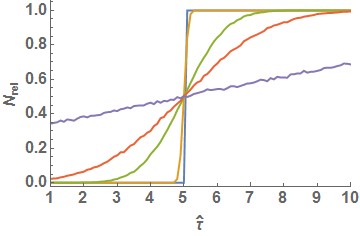
\includegraphics[width=.9\columnwidth]{../figures/thm2fig.png}
	\centering\caption{Visualization of Theorem~\ref{thrm:relativefrequency} as $N_{rel}$ estimates $\Phi(\cdot)$. The plot was generated by running Eqn.~\ref{eqn:Nrel} 10,000 times for each point in $\hat{\tau} = [1,10,\text{ (inc.) }0.1]$. $n = 10$, $\td = 5$ and $x_i = \hat{\tau} + \eta_i$ ($\eta_i \sim\mathcal{N}(0, \sigma)$). Each curve in the plot is generated by sweeping $\sigma = \{0, 0.1, 1, 2, 10\}$, with $\sigma = 0$ being a step-function and $\sigma = 10$ having the \emph{flattest} slope.}\vspace{-10px}\label{fig:thm2fig}
\end{figure}

Therefore, for large $n$, the relative frequency of agents taking part in the activity has a shape that follows the shape of the cdf of a standard Gaussian random variable, as seen in Fig.~\ref{fig:thm2fig}, i.e. agents may use deterministic threshold strategies but their aggregate behavior would appear to follow such a continues (sigmoid) threshold.

The final step to explain the prevalence of sigmoid functions in multiagent settings is to note that:
\begin{align*}
|\Phi(\frac{\hat{\tau}-\td}{\sigma^2})-\frac{1}{1+e^{-d(\frac{\hat{\tau}-\td}{\sigma^2})}}|\leq 0.01,
\end{align*}
for all $\hat{\tau}\in\R$ and some optimal value $d\approx 1.704$ (see \cite{camilli1994} and the references therein for the details of this approximation). This means that the aggregate behavior of the agents following deterministic threshold policies would (almost) follow the shape of a logistic sigmoid function whose drift is directly proportional to $\td$ and the slope  is inversely proportional to $\sigma^2$. 



\section{Discussion}\label{sec:disc}
We show in Theorem~\ref{thrm:mainthrm} that a communication-free agent-level threshold strategy is sufficient and necessary to achieve a task-allocation resulting in system-level equilibrium for concurrent benefit tasks. We then show in Theorem~\ref{thrm:relativefrequency} how such a policy effectively reduces to a continuous threshold response function that is commonly observed in social insects. While this result explains why we would observe such phenomena in natural systems, the game theory perspective leaves it unclear why one should choose a continuous threshold function in a robotic setting. Here, we would like to recall that a benefit of using a sigmoid vs.\ a step function is the randomness it adds, allowing swarm systems to quickly adapt to changes in task and environment parameters \cite{Bonabeau1997}. In particular, deliberately tuning the slope of the sigmoid threshold function as we have investigated in \cite{Kanakia2014} allows a swarm to explore different team sizes, and possibly learn from this experience, an aspect we wish to study in future work. 

Theorem~\ref{thrm:mainthrm} states that there exists a unique strategy profile $s$ such that it is a system-level Bayesian Nash Equilibrium for all agents performing a concurrent benefit task. Notice that this theorem makes no claims towards an \emph{optimal} strategy for task-assignment, just an equilibrium strategy. It is important to distinguish between these two properties of the swarm system. Clearly, optimal outcomes will require communication among agents or, at least, a central entity with access to global information. In future work, we wish to study the area inbetween in wich agents exchange limited amounts of information, such as their noisy estimates $x_i$, e.g.. In particular, we have shown elsewhere \cite{Touri2014}, that noisy sharing of information leads to non-existence of such an equilibrium.

This raises the question what ``communication'' and ``sharing of information'' actually mean. In this paper, communication is limited to common observations of an unknown environmental variable $\tau$. Natural swarming systems often communicate by modifying the environment, a form of indirect communication known as stigmergy \cite{grasse1959reconstruction}. The key difference between this form of communication and direct exchange of information, as we discuss in \cite{Touri2014}, is that the same information is simultaneously accessible to all individuals. We therefore believe that the results presented here extend also to indirect communication via stigmergy where $\tau$ is the measurable result of previous agent activity.

\section{Conclusion}\label{sec:conc}
We formulated robotic task-allocation in the context of game theory, and showed how a common class of tasks can be reduced to a global game. Using this framework we showed that a threshold-based policy, which is commonly observed in social insects and successfully used in swarm robotics, can indeed be considered an optimal policy if agents do not communicate. We also showed how such a policy reduced to a continuous response-threshold function that is commonly observed in natural systems under the influence of perception noise. While such a policy preserves a Bayesian Nash Equilibrium as the total number of agents increase, it also allows the system to balance between exploitation and exploration, thereby allowing the swarm flexibility to alter strategies for changing environmental parameters.

\section*{Acknowledgements}
We would like to thank Dana Hughes and John Klingner for their enlightening discussions on probability distributions and fixed point theory.

%%%%%%%%%%%%%%%%%%%%%%%%%%%%%%%%%%%%%%%%%%%%%%%%%%%%%%%%%%%%%%%%%%%%%%%%%%%%%%%%
%%%%%%%%%   The Bibliography, if any   %%%%%%%%%
\bibliographystyle{IEEEtran}		% or "siam", or "alpha", etc.
%\nocite{*}
\bibliography{../refworks}
\end{document}
